\documentclass{structure/itu-thesis}
\usepackage[utf8]{inputenc}
\usepackage{listings,xcolor}
\usepackage{xcolor}
\usepackage[scaled=0.9]{DejaVuSansMono}
\usepackage{listings}
\usepackage{graphicx}
\usepackage{tikz}
\usepackage{array}
\usepackage{commath}
\usepackage{physics}
\usepackage{amsmath}
\usepackage{afterpage}
\usepackage{tikz}
\usepackage{bigints}
\usepackage{mathdots}
\usepackage{yhmath}
\usepackage{cancel}
\usepackage{color}
\usepackage{siunitx}
\usepackage{array}
\usepackage{multirow}
\usepackage{amssymb}
\usepackage{gensymb}
\usepackage{tabularx}
\usepackage{booktabs}


%% Setting up the bibliography
\usepackage{biblatex}
\addbibresource{report.bib}

%% Additional packages and commands
\usepackage{hyperref}
\usepackage{fontawesome}
\setlist{itemsep=-2pt} % Reducing white space in lists slightly
\renewcommand{\deg}{\si{\degree}\xspace} % Use \deg easily, everywhere

%%%%%%%%%%%%%%%%%%%%%%%%%%%%%
%%%%% Begin of document %%%%%
%%%%%%%%%%%%%%%%%%%%%%%%%%%%%

\begin{document}

%% Roman page numbering
\frontmatter

%% Defining the main parameters
\title{A Title to the Report}
\subtitle{A Catchy Optional Subtitle \\ that Grabs the Attention}
\author{Your Full Name}

\newcommand{\documenttype}{Bachelor Thesis}
\newcommand{\thesistitle}{A Title to the Report}
\newcommand{\thesissubtitle}{A Catchy Optional Subtitle that Grabs the Attention}

\newcommand{\thesisauthor}{Your Full Name} % Your name :) 
\newcommand{\studentnumber}{090XXXXXX}
\newcommand{\thedate}{Date, year} % For example "June, 2022"

\newcommand{\department}{ITU Physics Engineering}
\newcommand{\departmentdescriber}{Faculty of Science and Letters}
\newcommand{\addressI}{ITU Ayazaga Campus, FEB Building}
\newcommand{\addressII}{34469 Maslak-Istanbul}
\newcommand{\departmentwebsite}{www.itu.edu.tr/en}

% Colours 
\newcommand{\targetcolourmodel}{cmyk} % rgb for a digital version, cmyk for a printed version. Only use lowercase
\selectcolormodel{\targetcolourmodel}

% Define colours from https://www.itu.edu.tr/hakkimizda#kimlik

\definecolor{navyblue}  {rgb/cmyk}{0, 0.267, 0.486 / 1.00, 0.45, 0.00, 0.51}
\definecolor{honeyyellow}  {rgb/cmyk}{0.706, 0.592, 0.349 / 0.00, 0.16, 0.51, 0.29}

\newcommand{\itulogocolour}{white} % Colour of the ITU logo: white, black
\newcommand{\frontpagetextcolour}{white} % front page text colour: white
\colorlet{frontbackcolor}{navyblue} % Set the background colour of the front- and back page.

\begin{titlepage}

\newgeometry{left=11mm,right=11mm,top=50mm,bottom=0pt}
\pagecolor{frontbackcolor}
\color{\frontpagetextcolour}

{ % Thesis title 
\Huge
\begin{tabular}{p{\linewidth}}
\textbf{\thesistitle}  \\ 
\LARGE{\thesissubtitle} \bigskip \\ 
{\huge \documenttype}
\end{tabular}
}

% ITU Department
\begin{tikzpicture}[remember picture,overlay]
\node[anchor=north east, 
      xshift=-10mm, 
      yshift=-12mm] 
      at (current page.north east) 
      {
        \color{\frontpagetextcolour}
        \begin{tabular}{r} 
        \large{\textbf{\thesisauthor}} \\ 
        \studentnumber
        \end{tabular}
      }; 
\end{tikzpicture}

% ITU logo
\begin{tikzpicture}[remember picture,overlay]
\node[anchor=north west, 
      xshift=8.9mm, 
      yshift=-8.3mm] 
     at (current page.north west) 
     {
\includegraphics[width=34.75mm,keepaspectratio]{structure/structure_figures/itu_white_logo.pdf}}; 
\end{tikzpicture}

% Thesis cover photo
\begin{tikzpicture}[remember picture,overlay]
\node[anchor=south, % anchor is bottom of picture
      xshift=0pt, 
      yshift=-2.9mm] % shifting picture to actually be at the bottom of the page
     at (current page.south) % placement at bottom of the page
     {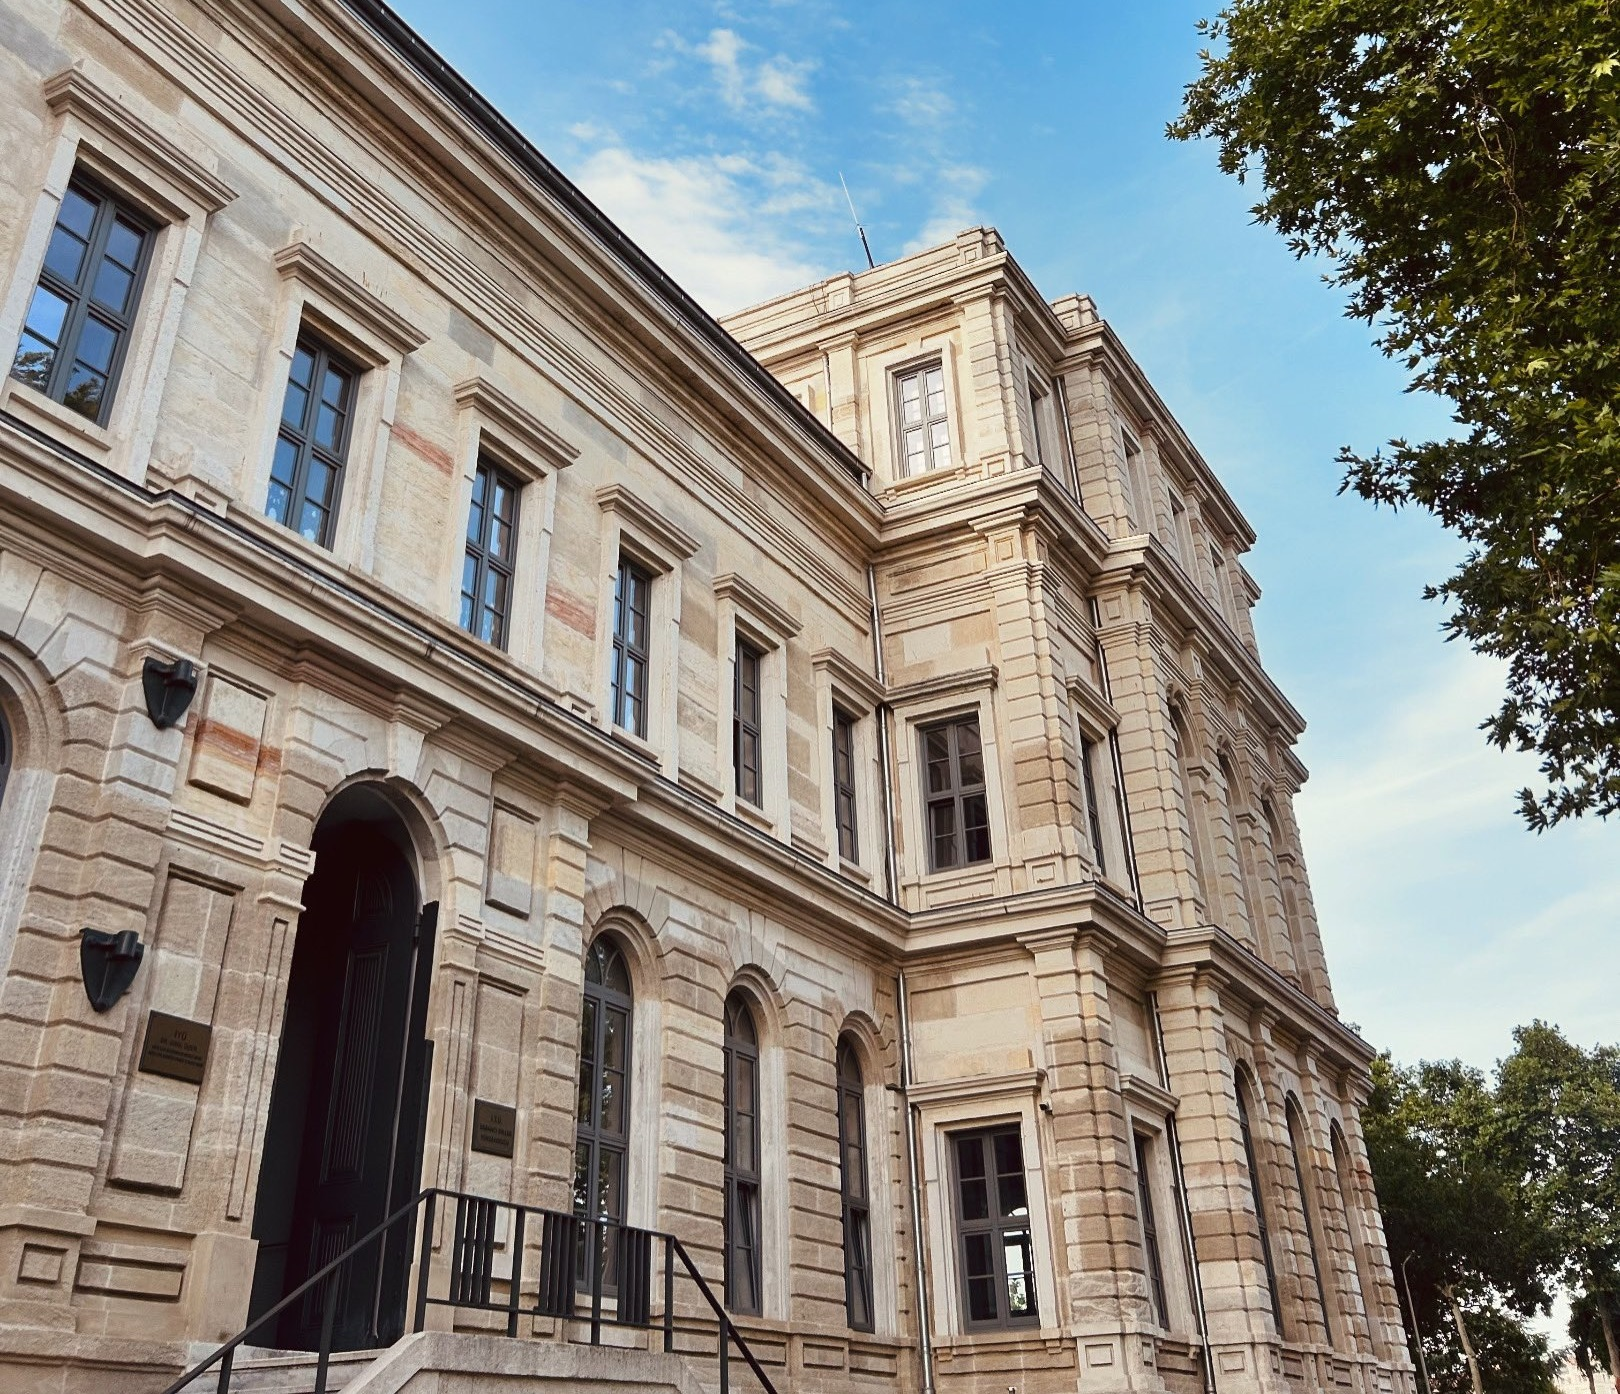
\includegraphics[height=18.9cm,keepaspectratio]{structure/structure_figures/itu_thesis_cover_photo.jpg}};
\end{tikzpicture}




\end{titlepage}
\afterpage{\nopagecolor}
\begin{titlepage}

\begin{center}

%% Print the title
{\makeatletter
\largetitlestyle\fontsize{45}{45}\selectfont\@title
\makeatother}

%% Print the subtitle
{\makeatletter
\ifdefvoid{\@subtitle}{}{\bigskip\titlestyle\fontsize{20}{20}\selectfont\@subtitle}
\makeatother}

\bigskip
\bigskip

by

\bigskip
\bigskip

%% Print the name of the author
{\makeatletter
\largetitlestyle\fontsize{25}{25}\selectfont\@author
\makeatother}

\bigskip
\bigskip

%% Print table with names and student numbers
\setlength\extrarowheight{2pt}

\vspace{3cm}

\begin{tabular}{c}
    Project Advisor \\\midrule
    Asst. Prof. XYZ XYZ (Faculty of Science and Letters, ITU) \\
\end{tabular}

\vspace{1cm}

\begin{tabular}{c}
    Jury Members \\\midrule
    ... \\
    ... \\
\end{tabular}

\vspace{4cm}

%% Print some more information at the bottom
\begin{tabular}{ll}
    Academic Semester: & Spring, 202X - 202X, \\
    Faculty: & Faculty of Science and Letters\\
    Thesis Submission Date : & ..., 202X\\
    Defense Date : & ..., 202X\\
\end{tabular}

\vspace{1cm}

%% Add a source and description for the cover and optional attribution for the template
\begin{tabular}{p{15mm}p{10cm}}
    Cover: & Lorem ipsum dolor sit amet, et quo eripuit oportere\\
\end{tabular}

\end{center}


%% Insert the ITU logo at the bottom of the page
\begin{tikzpicture}[remember picture, overlay]
    \node[above=10mm] at (current page.south) {%
        
\includegraphics[width=0.35\linewidth]{structure/structure_figures/itu_black_logo.pdf}
    };
\end{tikzpicture}

\end{titlepage}
\newgeometry{top=2.81cm, bottom=2.75cm, outer=2.5cm, inner=3.5cm}
\pagestyle{empty}
\cleardoublepage 


 \newpage

  \thispagestyle{empty} \mbox{}

  \vfill

  \begin{center}
    \textit{
      To the one whose clarity shines like the moon, bright as the moon and lighting my path
    }
  \end{center} \vspace*{5cm}

  \vfill 
\vspace*{-6pt}

For the foreword, 1 line spacing must be set. The foreword, written as a first page of the thesis must not exceed 2 pages. 

The acknowledgments must be given in this section.

After the foreword text, name of the author (right-aligned), and the date (as month and year) must be written (left-aligned). These two expressions must be in the same line. 

The foreword is written with 1 line spacing.

Lorem ipsum dolor sit amet, et quo eripuit oportere. Invenire urbanitas elaboraret cum no, eu vix saperet gubergren liberavisse. No eum doming iuvaret quaeque, alii perfecto mel in, an est liber aperiri vituperata. Mel an zril laoreet antiopam. Ne adolescens vituperata est, laudem altera eirmod sed ne, debet timeam aliquip mea no.

Vel euripidis delicatissimi et. Ea qui dictas quaeque voluptua. Ne modus movet inermis qui. Usu insolens torquatos suscipiantur ne. Duo ei nominavi consequat elaboraret, et tation sapientem pertinacia pri. Cu partiendo consequuntur est.

Ea vero possit aliquid est. Eos et illum nonumy quaestio, nec eu inani eripuit lobortis, ut eos inani copiosae senserit. Ut nec esse melius, id invenire mediocrem has, unum nostro scriptorem sit cu. Nostrum voluptua insolens duo id, cibo error viderer in duo, prodesset persequeris in quo. Ex mea stet adhuc, id per veniam praesent convenire, et cibo vitae duo. Qui enim exerci tincidunt ea. Nec eius assueverit ei, sit omnis ornatus ea, illum nemore id vel.
\chapter*{Preface}
\addcontentsline{toc}{chapter}{Preface}

Lorem ipsum dolor sit amet, et quo eripuit oportere. Invenire urbanitas elaboraret cum no, eu vix saperet gubergren liberavisse. No eum doming iuvaret quaeque, alii perfecto mel in, an est liber aperiri vituperata. Mel an zril laoreet antiopam. Ne adolescens vituperata est, laudem altera eirmod sed ne, debet timeam aliquip mea no.

Vel euripidis delicatissimi et. Ea qui dictas quaeque voluptua. Ne modus movet inermis qui. Usu insolens torquatos suscipiantur ne. Duo ei nominavi consequat elaboraret, et tation sapientem pertinacia pri. Cu partiendo consequuntur est.

Ea vero possit aliquid est. Eos et illum nonumy quaestio, nec eu inani eripuit lobortis, ut eos inani copiosae senserit. Ut nec esse melius, id invenire mediocrem has, unum nostro scriptorem sit cu. Nostrum voluptua insolens duo id, cibo error viderer in duo, prodesset persequeris in quo. Ex mea stet adhuc, id per veniam praesent convenire, et cibo vitae duo. Qui enim exerci tincidunt ea. Nec eius assueverit ei, sit omnis ornatus ea, illum nemore id vel.

Eu animal incorrupte qui. Usu amet explicari et, pro amet ullum sanctus cu. Quas semper ea his, dictas temporibus cu usu, facete pertinax argumentum ea vis. Ne detracto gubergren his, per eu noluisse conclusionemque. Eam falli docendi repudiare an. Dicta primis ei per, iudico iudicabit te eum.

Debitis constituto reformidans ad mea, mea tation decore maiorum an. Delicata recteque et usu, enim esse recusabo sea ei, ex natum justo quo. Ea per postulant salutatus conceptam. Tempor iriure eligendi vix an, similique moderatius ea nam.

\begin{flushright}
{\makeatletter\itshape
    \@author \\
    Istanbul, \monthname{} \the\year{}
\makeatother}
\end{flushright}
\tableofcontents
\listoffigures
\listoftables

\chapter*{Nomenclature}
\addcontentsline{toc}{chapter}{Nomenclature}


\section*{Abbreviations}

\begin{longtable}{p{2.5cm}p{8cm}}
    \toprule
    Abbreviation & Definition \\
    \midrule\endhead % Add abbreviations alphabetically here:
    BPM & Beam Propagation Method \\
    DOF & Depth of Focus  \\
    FFT & Fast Fourier Transform\\
    LD & Laser Diode \\
    \bottomrule
\end{longtable}

\section*{Symbols}

\begin{longtable}{p{2.5cm}p{8cm}p{2.5cm}}
    \toprule
    Symbol & Definition & Unit \\
    \midrule\endhead % Add Latin symbols alphabetically here:
    $B$ & Magnetic Field & [Tesla] \\
    $c$ & Speed of Light & [m/s] \\
    $D$ & Electric Displacement Field & [$C/m^2$] \\
    $E$ & Electric Field & [V/m] \\
    $I$ & Intensity & [$V/m^2$] \\
    $J$ & Current Density & [$A/m^2$] \\
    $J_m$ & Bessel functions of the first kind &  \\
    $P$ & Power & [W] \\
    \midrule % Add Greek symbols alphabetically here:
    $\rho$ & Charge Density & [$C/m^3$] \\
    $\epsilon_0$ & Vacuum Permittivity & [F/m] \\
    $\mu_0$ & Vacuum Permeability & [$m kg / s^2 A^2$] \\
    \bottomrule
\end{longtable}

%% ----------------------------------------------------------------------
%%    Mainmatter (Arabic page numbering)
%% ----------------------------------------------------------------------

\mainmatter

\chapter{Chapter 1}
\label{chapter:introduction}

Lorem ipsum dolor sit amet, et quo eripuit oportere. Invenire urbanitas elaboraret cum no, eu vix saperet gubergren liberavisse. No eum doming iuvaret quaeque, alii perfecto mel in, an est liber aperiri vituperata. Mel an zril laoreet antiopam. Ne adolescens vituperata est, laudem altera eirmod sed ne, debet timeam aliquip mea no.

Vel euripidis delicatissimi et. Ea qui dictas quaeque voluptua. Ne modus movet inermis qui. Usu insolens torquatos suscipiantur ne. Duo ei nominavi consequat elaboraret, et tation sapientem pertinacia pri. Cu partiendo consequuntur est.

Ea vero possit aliquid est. Eos et illum nonumy quaestio, nec eu inani eripuit lobortis, ut eos inani copiosae senserit. Ut nec esse melius, id invenire mediocrem has, unum nostro scriptorem sit cu. Nostrum voluptua insolens duo id, cibo error viderer in duo, prodesset persequeris in quo. Ex mea stet adhuc, id per veniam praesent convenire, et cibo vitae duo. Qui enim exerci tincidunt ea. Nec eius assueverit ei, sit omnis ornatus ea, illum nemore id vel.
\chapter{Chapter 2}
\label{chapter:maintext1}


%\begin{figure}[h]
%    \centering
%    \includegraphics[width=0.95\linewidth]{figures/template.png}
%    \caption{Preview of the template}
%\end{figure}

Lorem ipsum dolor sit amet, et quo eripuit oportere. Invenire urbanitas elaboraret cum no, eu vix saperet gubergren liberavisse. No eum doming iuvaret quaeque, alii perfecto mel in, an est liber aperiri vituperata. Mel an zril laoreet antiopam. Ne adolescens vituperata est, laudem altera eirmod sed ne, debet timeam aliquip mea no.

Vel euripidis delicatissimi et. Ea qui dictas quaeque voluptua. Ne modus movet inermis qui. Usu insolens torquatos suscipiantur ne. Duo ei nominavi consequat elaboraret, et tation sapientem pertinacia pri. Cu partiendo consequuntur est.

Ea vero possit aliquid est. Eos et illum nonumy quaestio, nec eu inani eripuit lobortis, ut eos inani copiosae senserit. Ut nec esse melius, id invenire mediocrem has, unum nostro scriptorem sit cu. Nostrum voluptua insolens duo id, cibo error viderer in duo, prodesset persequeris in quo. Ex mea stet adhuc, id per veniam praesent convenire, et cibo vitae duo. Qui enim exerci tincidunt ea. Nec eius assueverit ei, sit omnis ornatus ea, illum nemore id vel.
\chapter{Chapter 3}
\label{chapter:maintext2}

Lorem ipsum dolor sit amet, et quo eripuit oportere. Invenire urbanitas elaboraret cum no, eu vix saperet gubergren liberavisse. No eum doming iuvaret quaeque, alii perfecto mel in, an est liber aperiri vituperata. Mel an zril laoreet antiopam. Ne adolescens vituperata est, laudem altera eirmod sed ne, debet timeam aliquip mea no.

Vel euripidis delicatissimi et. Ea qui dictas quaeque voluptua. Ne modus movet inermis qui. Usu insolens torquatos suscipiantur ne. Duo ei nominavi consequat elaboraret, et tation sapientem pertinacia pri. Cu partiendo consequuntur est.

Ea vero possit aliquid est. Eos et illum nonumy quaestio, nec eu inani eripuit lobortis, ut eos inani copiosae senserit. Ut nec esse melius, id invenire mediocrem has, unum nostro scriptorem sit cu. Nostrum voluptua insolens duo id, cibo error viderer in duo, prodesset persequeris in quo. Ex mea stet adhuc, id per veniam praesent convenire, et cibo vitae duo. Qui enim exerci tincidunt ea. Nec eius assueverit ei, sit omnis ornatus ea, illum nemore id vel.

\section{Section 1}\label{section1}

Lorem ipsum dolor sit amet, et quo eripuit oportere. Invenire urbanitas elaboraret cum no, eu vix saperet gubergren liberavisse. No eum doming iuvaret quaeque, alii perfecto mel in, an est liber aperiri vituperata. Mel an zril laoreet antiopam. Ne adolescens vituperata est, laudem altera eirmod sed ne, debet timeam aliquip mea no.

Vel euripidis delicatissimi et. Ea qui dictas quaeque voluptua. Ne modus movet inermis qui. Usu insolens torquatos suscipiantur ne. Duo ei nominavi consequat elaboraret, et tation sapientem pertinacia pri. Cu partiendo consequuntur est.

Ea vero possit aliquid est. Eos et illum nonumy quaestio, nec eu inani eripuit lobortis, ut eos inani copiosae senserit. Ut nec esse melius, id invenire mediocrem has, unum nostro scriptorem sit cu. Nostrum voluptua insolens duo id, cibo error viderer in duo, prodesset persequeris in quo. Ex mea stet adhuc, id per veniam praesent convenire, et cibo vitae duo. Qui enim exerci tincidunt ea. Nec eius assueverit ei, sit omnis ornatus ea, illum nemore id vel.

\subsection{Subsection 1}

Lorem ipsum dolor sit amet, et quo eripuit oportere. Invenire urbanitas elaboraret cum no, eu vix saperet gubergren liberavisse. No eum doming iuvaret quaeque, alii perfecto mel in, an est liber aperiri vituperata. Mel an zril laoreet antiopam. Ne adolescens vituperata est, laudem altera eirmod sed ne, debet timeam aliquip mea no.

Vel euripidis delicatissimi et. Ea qui dictas quaeque voluptua. Ne modus movet inermis qui. Usu insolens torquatos suscipiantur ne. Duo ei nominavi consequat elaboraret, et tation sapientem pertinacia pri. Cu partiendo consequuntur est.

Ea vero possit aliquid est. Eos et illum nonumy quaestio, nec eu inani eripuit lobortis, ut eos inani copiosae senserit. Ut nec esse melius, id invenire mediocrem has, unum nostro scriptorem sit cu. Nostrum voluptua insolens duo id, cibo error viderer in duo, prodesset persequeris in quo. Ex mea stet adhuc, id per veniam praesent convenire, et cibo vitae duo. Qui enim exerci tincidunt ea. Nec eius assueverit ei, sit omnis ornatus ea, illum nemore id vel.

\begin{itemize}
	\setlength{\itemindent}{-0.35em} % Flush the bullets to the left
	\item{Figures, tables can be enlarged and be reduced.}
	\vspace{-3mm}
	\item{The explanations except from the first reference about the figure or table can be placed either before the figure/table or after.}
	\vspace{-3mm}
	\item{After referring to a figure or table it is placed to the closest and convenient location. Convenient location must be arranged considering the gap at the bottom of the page.}
\end{itemize}

\begin{figure}
%\begin{sidewaysfigure}
	\centering
	\includegraphics[width=280pt,keepaspectratio=true]{./fig/sekil3}
	% sekil3.eps: 0x0 pixel, 300dpi, 0.00x0.00 cm, bb=14 14 1155 740
	\caption{Neuron cell, adapted from (\c{C}etin, 2003).}
	\label{Figure3.1}
%\end{sidewaysfigure}
\end{figure}

Lorem ipsum dolor sit amet, et quo eripuit oportere. Invenire urbanitas elaboraret cum no, eu vix saperet gubergren liberavisse. No eum doming iuvaret quaeque, alii perfecto mel in, an est liber aperiri vituperata. Mel an zril laoreet antiopam. Ne adolescens vituperata est, laudem altera eirmod sed ne, debet timeam aliquip mea no.

Vel euripidis delicatissimi et. Ea qui dictas quaeque voluptua. Ne modus movet inermis qui. Usu insolens torquatos suscipiantur ne. Duo ei nominavi consequat elaboraret, et tation sapientem pertinacia pri. Cu partiendo consequuntur est.

Ea vero possit aliquid est. Eos et illum nonumy quaestio, nec eu inani eripuit lobortis, ut eos inani copiosae senserit. Ut nec esse melius, id invenire mediocrem has, unum nostro scriptorem sit cu. Nostrum voluptua insolens duo id, cibo error viderer in duo, prodesset persequeris in quo. Ex mea stet adhuc, id per veniam praesent convenire, et cibo vitae duo. Qui enim exerci tincidunt ea. Nec eius assueverit ei, sit omnis ornatus ea, illum nemore id vel.

\subsection{Subsection 2}

Lorem ipsum dolor sit amet, consetetur sadipscing elitr, sed diam nonumy eirmod tempor invidunt ut labore et dolore magna aliquyam erat, sed diam voluptua. At vero eos et accusam et justo duo dolores et ea rebum. Stet clita kasd gub rgren, no sea takimata sanctus est  Lorem ipsum dolor sit amet, consetetur sadipscing elitr, sed diam nonumy eirmod tempor invidunt ut lab  ore sit et dolore magna equation (\ref{Eq3.1}).
\begin{equation}
y_{t} = \phi_{1} y_{t-1} + \epsilon_{t}
\label{Eq3.1}
\end{equation}
Lorem ipsum dolor sit amet, consetetur sadipscing elitr, sed diam nonumy eirmod tempor invidunt ut labore et dolore magna aliquyam erat, sed diam voluptua. At vero eos et accusam et justo duo dolores et ea rebum. Stet clita kasd gub rgren, no sea takimata sanctus est Lorem ipsum dolor sit amet, consetetur sadipscing elitr, sed diam nonumy eirmod tempor invidunt ut lab ore sit et dolore magna.
% Subequation example - SBÖ
\vskip -24pt
\begin{subequations}
	\begin{gather}
	R_0 = 0 \label{Eq3.2a}\\
	N_0 = 0 \label{Eq3.2b}
	\end{gather}
	\label{Eq3.2ab}
\end{subequations}
\vskip -24pt

Lorem ipsum dolor sit amet, et quo eripuit oportere. Invenire urbanitas elaboraret cum no, eu vix saperet gubergren liberavisse. No eum doming iuvaret quaeque, alii perfecto mel in, an est liber aperiri vituperata. Mel an zril laoreet antiopam. Ne adolescens vituperata est, laudem altera eirmod sed ne, debet timeam aliquip mea no.


\subsection{Subsection 3}

Lorem ipsum dolor sit amet, consetetur sadipscing elitr, sed diam nonumy eirmod tempor invidunt ut labore et dolore magna aliquyam erat, sed diam voluptua. At vero eos et accusam et justo duo dolores et ea rebum. Stet clita kasd gub rgren, no sea takimata sanctus est Lorem ipsum dolor sit amet, consetetur sadipscing elitr, sed diam nonumy eirmod tempor invidunt ut lab ore sit et dolore magna.

Lorem ipsum dolor sit amet, consetetur sadipscing elitr, sed diam nonumy eirmod tempor invidunt ut labore et dolore magna aliquyam erat, sed diam voluptua. At vero eos et accusam et justo duo dolores et ea rebum. Stet clita kasd gub rgren, no sea takimata sanctus est Lorem ipsum dolor sit amet, consetetur sadipscing elitr, sed diam nonumy eirmod tempor invidunt ut lab ore sit et dolore magna.

\begin{figure}
	\centering
	\includegraphics[width=250pt,keepaspectratio=true]{./fig/sekil3}
	% sekil3.eps: 0x0 pixel, 300dpi, 0.00x0.00 cm, bb=14 14 1155 740
	\caption{For a multi-line figure captions, it is important that all the lines of the caption are aligned.}
	\label{Figure3.2}
\end{figure}





%% Prevent urls running into margins in bibliography
\setcounter{biburlnumpenalty}{7000}
\setcounter{biburllcpenalty}{7000}
\setcounter{biburlucpenalty}{7000}

%% ----------------------------------------------------------------------
%%    Appendix (Letters for chapters)
%% ----------------------------------------------------------------------

\backmatter
\chapter{Source Code Example}
%\label{chapter:title}

{\normalfont\texttt{listings}}. An example can be found below. Files can be added using \\ {\normalfont\texttt{\textbackslash lstinputlisting[language=<language>]\{<filename>\}}}

\begin{lstlisting}[language=Python]
import jax
import jax.numpy as jnp
import optax
from jax import grad, jit, vmap
from jax.scipy.special import logsumexp
from typing import Callable, Tuple

# Generate a random adjacency matrix for a graph
def generate_random_graph(num_nodes: int, edge_prob: float) -> jnp.ndarray:
    """Generates a random adjacency matrix for a graph with given probability of edge existence."""
    rng = jax.random.PRNGKey(0)
    adjacency_matrix = jax.random.bernoulli(rng, p=edge_prob, shape=(num_nodes, num_nodes))
    adjacency_matrix = jnp.triu(adjacency_matrix, 1)  # Upper triangular to avoid self-loops
    adjacency_matrix = adjacency_matrix + adjacency_matrix.T  # Symmetrize
    return adjacency_matrix

# Define the graph coloring loss function
def graph_coloring_loss(colors: jnp.ndarray, adjacency_matrix: jnp.ndarray) -> jnp.ndarray:
    """Computes the loss function for the graph coloring problem."""
    num_nodes = adjacency_matrix.shape[0]
    color_matrix = jnp.expand_dims(colors, 0) == jnp.expand_dims(colors, 1)
    adjacency_loss = jnp.sum(adjacency_matrix * color_matrix)
    return adjacency_loss

# Define the optimization step
def update(params: jnp.ndarray, opt_state: optax.OptState, grads: jnp.ndarray, optimizer: optax.GradientTransformation) -> Tuple[jnp.ndarray, optax.OptState]:
    """Updates parameters using Optax optimizer."""
    updates, opt_state = optimizer.update(grads, opt_state, params)
    return optax.apply_updates(params, updates), opt_state

# Main function to solve the graph coloring problem
def graph_coloring(num_nodes: int, edge_prob: float, num_colors: int, learning_rate: float, num_steps: int):
    adjacency_matrix = generate_random_graph(num_nodes, edge_prob)
    
    # Initialize color assignments randomly
    init_colors = jax.random.randint(jax.random.PRNGKey(1), shape=(num_nodes,), minval=0, maxval=num_colors)
    
    # Define the optimizer
    optimizer = optax.adam(learning_rate)
    
    # Define the loss function
    loss_fn = lambda colors: graph_coloring_loss(colors, adjacency_matrix)
    
    # Initialize optimizer state
    opt_state = optimizer.init(init_colors)
    
    # Gradient function
    grad_fn = jit(grad(loss_fn))
    
    # Optimization loop
    colors = init_colors
    for step in range(num_steps):
        grads = grad_fn(colors)
        colors, opt_state = update(colors, opt_state, grads, optimizer)
        
        # Print progress
        if step % 100 == 0:
            current_loss = loss_fn(colors)
            print(f"Step {step}, Loss: {current_loss:.2f}")

    return colors

# Parameters
num_nodes = 10
edge_prob = 0.3
num_colors = 3
learning_rate = 0.01
num_steps = 1000

# Run the graph coloring optimization
optimized_colors = graph_coloring(num_nodes, edge_prob, num_colors, learning_rate, num_steps)
print("Optimized Colors:", optimized_colors)
\end{lstlisting}
\chapter{Task Division Example}
%\label{chapter:title}

\emph{If a task division is required, a simple template can be found below for convenience. Feel free to use, adapt or completely remove.}

\begin{table}[htb]
    \setlength\extrarowheight{4pt}
    \centering
    \caption{Distribution of the workload}
    \label{tab:taskdivision}
    \begin{tabularx}{\textwidth}{lXX}
        \toprule
        & Task & Student Name(s) \\
        \midrule
        & Summary & \\
        Chapter 1 & Introduction &  \\
        Chapter 2 &  & \\
        Chapter 3 &  & \\
        Chapter * &  & \\
        Chapter * & Conclusion &  \\
        \midrule
        & Editors & \\
        & CAD and Figures & \\
        & Document Design and Layout & \\
        \bottomrule
    \end{tabularx}
\end{table}
%\input{appendix/appendix-c} % Create file to add

%% Add bibliography
\printbibliography[heading=bibintoc,title=References]

% Define colours from https://www.itu.edu.tr/hakkimizda#kimlik

\definecolor{navyblue}  {rgb/cmyk}{0, 0.267, 0.486 / 1.00, 0.45, 0.00, 0.51}
\definecolor{honeyyellow}  {rgb/cmyk}{0.706, 0.592, 0.349 / 0.00, 0.16, 0.51, 0.29}


\colorlet{frontbackcolor}{navyblue} % Set the background colour of the front- and back page. Choose the colour so it matches the main colour of front page picture

\newgeometry{left=15mm,right=14mm,top=50mm,bottom=14mm}
\thispagestyle{empty}
\pagecolor{frontbackcolor}
\color{white}

Lorem ipsum dolor sit amet, et quo eripuit oportere. Invenire urbanitas elaboraret cum no, eu vix saperet gubergren liberavisse. No eum doming iuvaret quaeque, alii perfecto mel in, an est liber aperiri vituperata. Mel an zril laoreet antiopam. Ne adolescens vituperata est, laudem altera eirmod sed ne, debet timeam aliquip mea no.

Vel euripidis delicatissimi et. Ea qui dictas quaeque voluptua. Ne modus movet inermis qui. Usu insolens torquatos suscipiantur ne. Duo ei nominavi consequat elaboraret, et tation sapientem pertinacia pri. Cu partiendo consequuntur est.

\vspace*{\fill}



\begin{tabular}{@{}l}
    Istanbul \\ 
    Technical \\ 
    University \\
    \\
    \addressI \\
    \addressII \\
    \\
    \url{\departmentwebsite}
\end{tabular}
\end{document}
